\begin{homeworkProblem}[Quiz 3, Pr. 1]
        Alright, you guys, let's go through this quiz that you did last
        week. It seemed to be a point of struggle for a number of
        you. I'll treat these problems in order and I will supply you
        with the problem statements that you were given on the quiz.

    \begin{homeworkSection}{1a}
        \textbf{A point charge is placed inside of a cube of side L,
        then inside of a sphere of radius L/2, then inside a cyliner of
        radius L/2 and height L. Which case will produce the highest
        [electric] flux through the above volumes individually?}
        \\

        Okay, so the trick with this problem is to understand what
        electric flux is. Electric flux is a measure of the amount of
        electric field lines that permeate a surface. For a stronger
        source of the electric field (like a larger charge or more
        charges) then the electric field will be greater at a given
        point in space. In order to measure the electric flux, though,
        we need to consider a surface. 
        
        See, the electric flux is a measure of how much electric field
        permeates a surface. So, we need something (a sheet, a sphere, a
        cube, etc.) which the electric field vectors will pierce. The
        electric flux through the surface will be a measure of the
        strength of the electric field directed through that surface.
        Mathematically, this is expressed as:
        
        \[
        \text{Electric flux} = \oint\limits_{\text{surface}}
        \vec{E}\cdot\vec{da} = \oint\limits_{\text{surface}} |\vec{E}|
        |\vec{da}| \cos\theta 
        \]
     
        \begin{figure}[t]
            \centering
            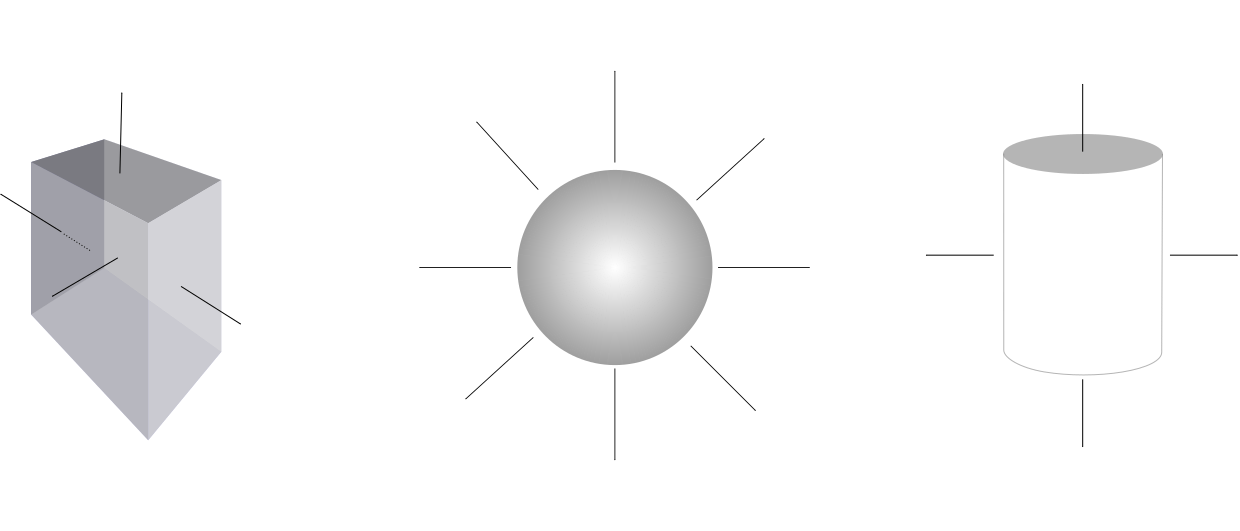
\includegraphics[width=.75\textwidth]{./img/davectors.pdf}
            \caption{$\diff a$ vectors for many common shapes
            Note that the direction of the $\diff a$ vector
            depends on where on the surface you are.}
            \label{fig:davectors.eps}
        \end{figure}

        What is that $\vec{da}$ quantity? Well, it's the vector that
        points normal to the surface at the point you are interested in
        (see %\ref{fig:davectors.eps}) If the surface that you're
        considering is closed (that is, it is a closed volume, unlike a
        sheet or something with a hole in it) then the area vector is
        defined to point normal to the surface and exterior to that
        surface. That is, it points to the outside of the surface. For
        an open surface (like a sheet) the area vector can be defined as
        normal to the surface in one of two directions (up or down, for
        a sheet). It must be specified which direction someone is
        considering when they specify a solution to a problem.
        
        See, the integral is calculated over the surface where you're
        looking at the electric field. The $\vec{da}$ vector is defined
        to be perpendicular to the surface. This might mean that it
        might have different $\hat{x}$ and $\hat{y}$ coordinates at
        different points in space (like for a sphere). But, it will
        always be perpendicular to the surface. The electric field, at
        the surface, may not be perpendicular to the surface. So, there
        may be an angle between the two vectors. In this case, the dot
        product becomes important.

        The dot product in that expression accounts for the fact that
        the electric field might not be piercing the surface in the same
        direction as the area vector. See, if the electric field is not
        parallel to the area vector at the surface %ref{fig:areavec.eps}
        then the amount of flux through that surface, the amount of
        electric field which passes through that surface is reduced.
        Think about it like this: If the electric field was
        perpendicular to the area vector at the surface then none of the
        electric field would pass through the surface.
        
        An oft-cited analogy for electric flux is the water that flows
        through a shower head. The amount of water that flows through
        the head of the shower can be thought of as the amount of
        electric field lines that penetrate a surface. If the water
        flows perpendicular through the surface then there will be no
        ``water flux''. The way in which to get the largest volume of
        water to pass through the surface is to align the water flow
        perpendicular to the surface. This is the same way in which
        electric flux is maximized: By being perpendicular to the
        surface.

        Okay, now that we've established what flux is qualiatively and
        quantitatively let's relate it to a quantity that's easier to
        measure: electric charge. It would be extremely difficult for
        most cases to calculate $\oint \vec{E}\cdot \vec{da}$. The
        electric field might not have a nice relationship with the area
        vector. The prototypical example is the case of a charge placed
        in the center of a cube. The electric field from the charge will
        be in the $\hat{r}$ direction. Thus, immediately above the
        charge, the electric field will point in the $\hat{z}$
        direction. But, off to the side, above the charge (for non-zero
        x and y coordinates), the direction of the electric field will
        havea non-zero x and y component. The top face of the cube,
        however, has an area vector that always points in the $+\hat{z}$
        direction. Thus, the angle between the electric field and the
        area vector will change over the whole surface of the cube. The
        expression for this, while possible to write, is difficult
        enough to make us want to find the magnitude of the electric
        flux in another way. It turns out, that the electric flux is
        related to the charge inside of a volume through the simple
        relationship:

        \[
        \Phi = \frac{Q_{enc}}{\epsilon_0}
        \]

        This is incredible! It tells us that if we want to calculate the
        flux and we happen to know the amount of enclosed charge inside
        the volume in which we're interested, we can just add that up
        and divide by $\epsilon_0$, the permittivity of free space, and
        we're done! The change outside of our volume has absolutely no
        effect on the electric flux through our surface! (I hate
        explanation points, but hopefully these help drive the
        importance of this result to you guys.)

        Now, let's think about the problem. We are asked to compare the
        amount of flux through each of the various surfaces. All of the
        closed surfaces (the cube, the sphere and the cylinder) have the
        exact same amount of charge enclosed inside of them. Thus,
        expression $\frac{Q_{enc}}{\epsilon_0}$ must be the same for all
        of them. Thus, the electric flux generated through each of the
        surfaces must be exactly the same. This is the answer.

    \end{homeworkSection}

    \begin{homeworkSection}{1b}
        \textbf{A point charge is placed at the center of a cube of side
        L. What is the flux through one of the faces?}
        \\

        \begin{figure}[t]
            \centering
            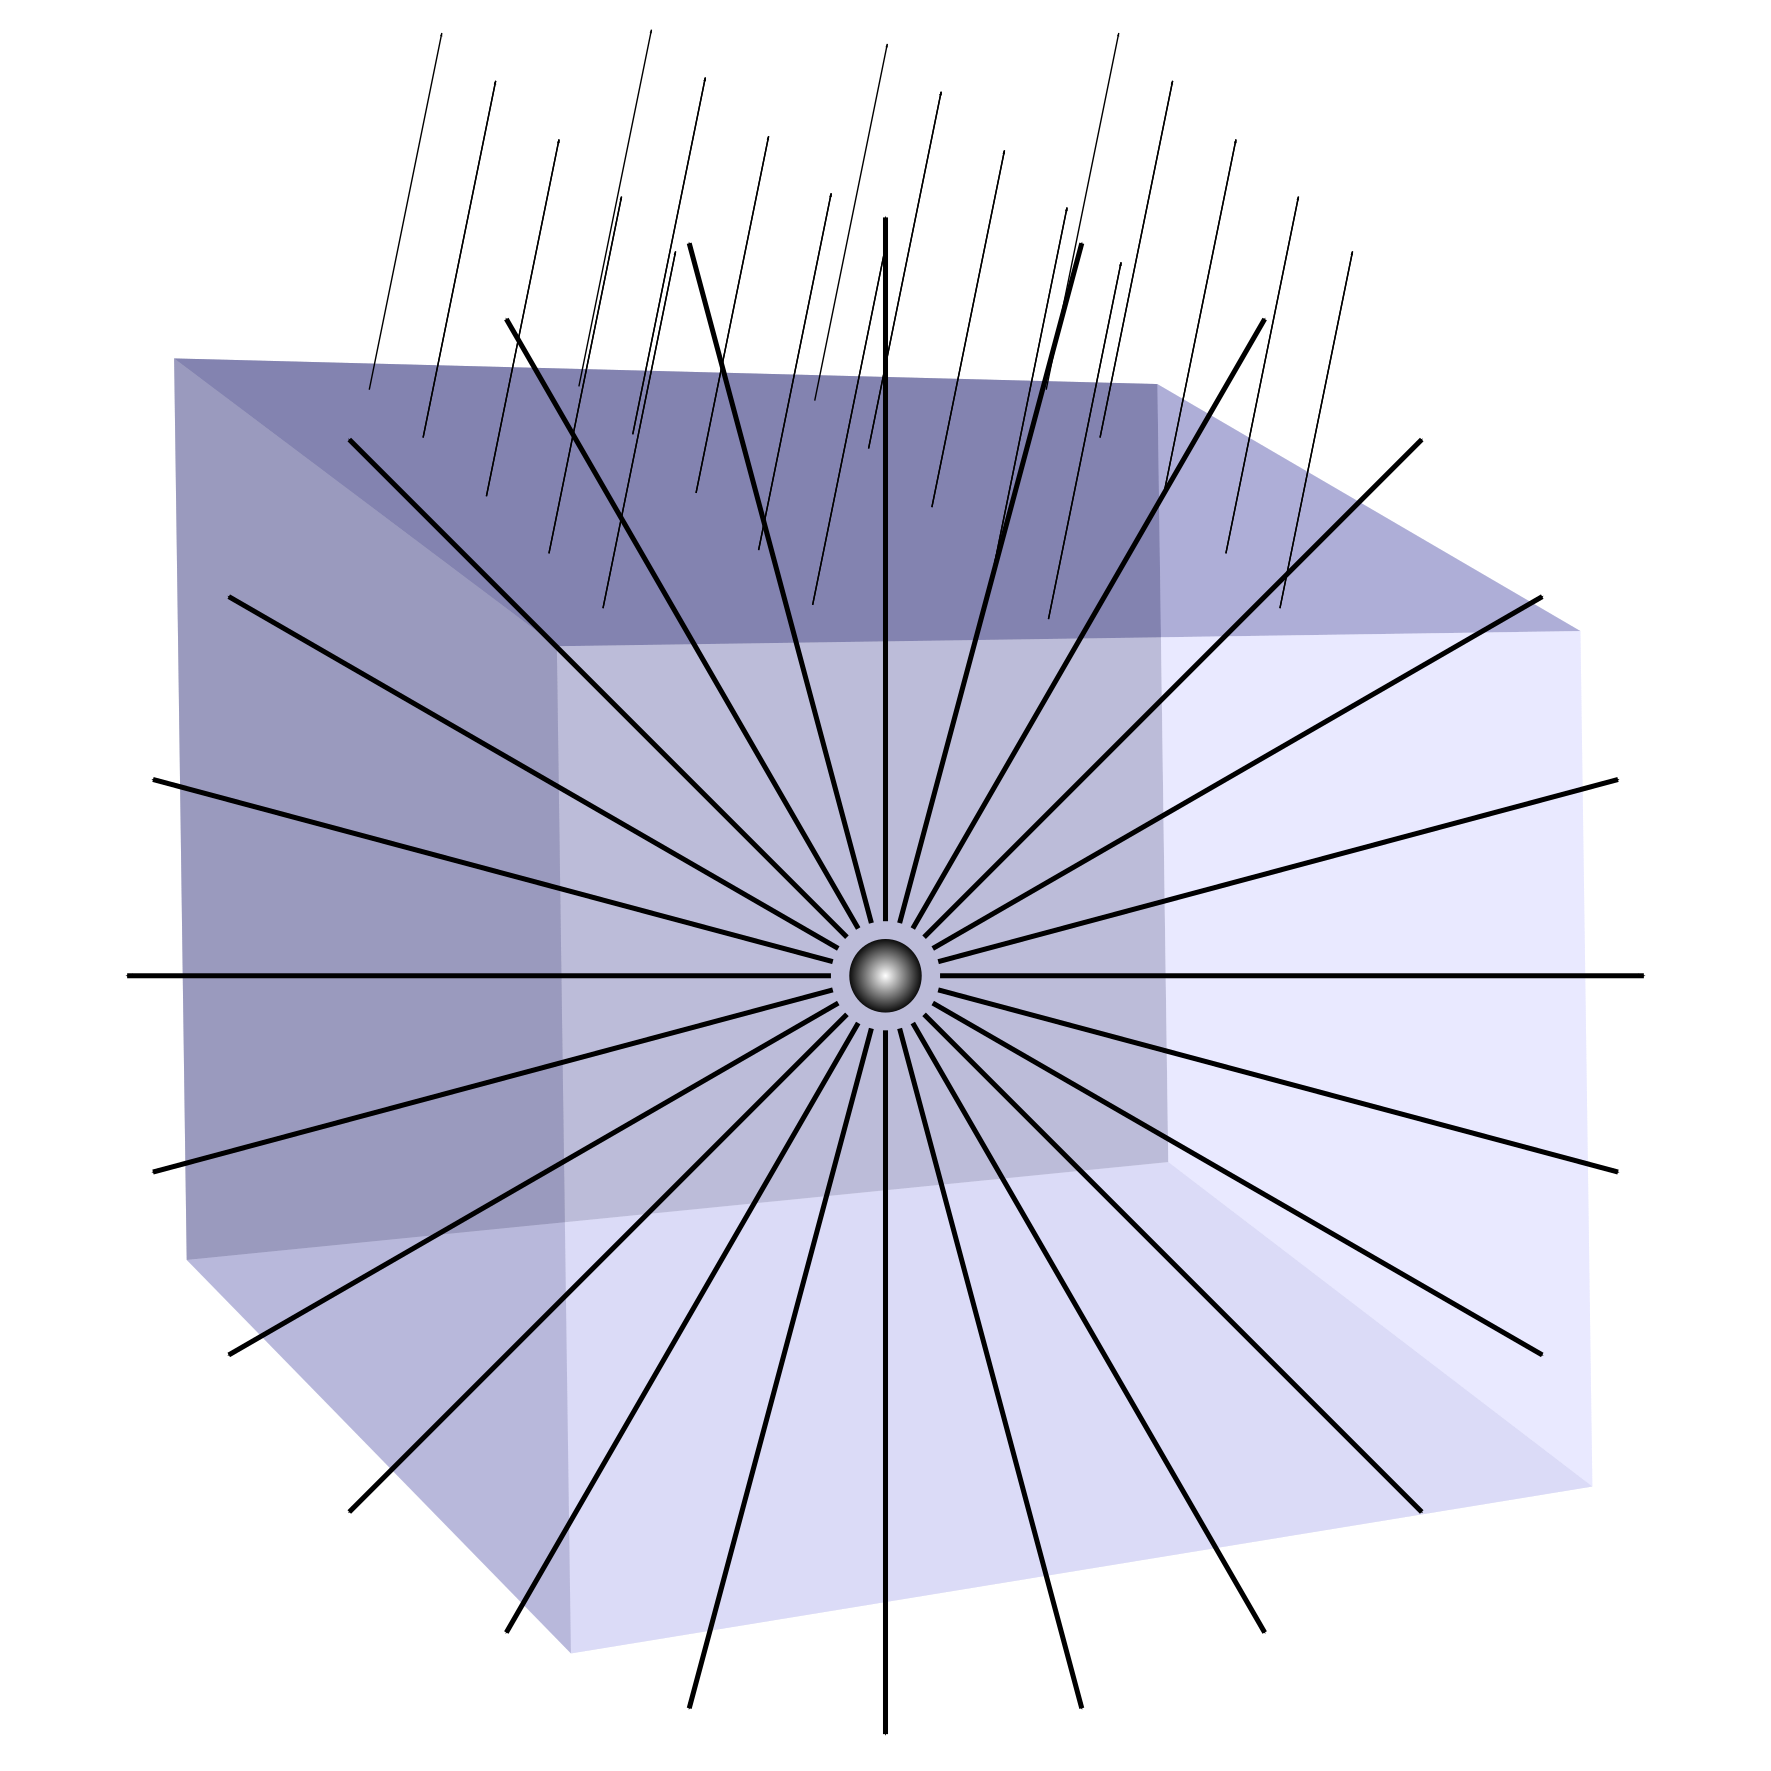
\includegraphics[width=.4\textwidth]{./img/chargeinbox.pdf}
            \caption{Figure depicting the electric field generated by a
            point charge in a box (area vectors of the top of the box
            shown above the point charge}
            \label{fig:chargeinbox.eps}
        \end{figure}

        Okay, the trick to this problem is to neglect the dimensions of
        the cube. We know that the enclosed charge determines thet total
        flux through the surface. Thus, we know that the total flux
        through the surface is $\Phi = \frac{Q}{\epsilon_0}$, where $Q$
        is the charge that is placed at the center of the cube. Now, if
        the charge is placed in the center, there is symmetry in the
        problem.
        
        For example, consider the left and right sides of the cube (see
        figure \ref{fig:chargeinbox.eps}). The amount of electric field
        and the direction of the electric field at the left and the
        right faces of the cube are exactly the same magnitude but in
        the opposite direction. So, $\vec{E}$ flips direction based on
        whether you're considering the right or left side of the cube.
        But, so does $\vec{da}$, the vector normal to the surface of the
        cube. Thus, the dot product is the same: $-\vec{E}\cdot\vec{-da}
        =\vec{E}\cdot\vec{da}$.

        Now, I could perform the same argument with the top and bottom
        and the front and back of the cube. Thus, there is symmetry with
        respect to three pairs of the cube's faces. Now, if I rotate the
        cube so that the right side becomes the top side I have the same
        electric field and the same $\vec{da}$ vectors. I can do this to
        show that the electric flux through each of the 6 faces of the
        cube is the exact same. Thus $\Phi = 6\Phi_{face} =
        \frac{Q}{\epsilon_0}$. So, finally:

        \[
        \Phi_{face} = \frac{Q}{6\epsilon_0}
        \]

        This is the answer to 1b.
    \end{homeworkSection}

    \begin{homeworkSection}{1c}
        \textbf{A point charge Q is placed inside the hemispherical
        Gaussian surface a distance $\delta$ from the flat face, as
        shown. Find the flux through the flat face in the limit as
        $\delta$ as goes to zero?}
        \\

        Let's consider this problem in the following way. There are a
        number of ways to justify the answer for this question. I like
        the following argument: The total flux through the surface is
        the sum of the flux through the flat face and the flux through
        the curved face: $\Phi = \Phi_{\text{curved face}}+
        \Phi_{\text{flat face}} $.
        
        However, the amount of flux through
        the curved face is one half the amount of flux that would go
        through an entire sphere. Notice that I can only say this in the
        limit as the charge goes infinitesimally close to the flat face.
       
        If the charge was far from the flat face then it would not look
        like the charge was at the center of a sphere to the hemisphere.
        If it's not at the center of the hemisphere then we can't simply
        say that the electric flux through the surface would be one half
        of that through the sphere, since the eletric field distribution
        with respect to the hemisphere changes drastically.

        Another way to say it is that as the charge gets close to the
        hemisphere (far from the flat face) more electric fields go
        through the flat face and less goes through the hemisphere since
        the electric field lines generated by the point charge would not
        be in the same direction as the area vector on the hemisphere
        ($\vec{da_{\text{hemisphere}}} = da \hat{r}$).

        Thus, since the entire flux through a sphere would be $\Phi =
        \frac{Q}{\epsilon_0}$, the flux through the hemisphere would be
        $\frac{Q}{2\epsilon_0}$. Thus, the flux through the flat face
        would be:

        \[ \Phi - \Phi_{\text{curved face}} = \frac{Q}{\epsilon_0} -
        \frac{Q}{2\epsilon_0} = \frac{Q}{2\epsilon_0} \]

        This is the question to 1c.

    \end{homeworkSection}
\end{homeworkProblem}
